\documentclass[a4paper, oneside]{memoir}
\usepackage[utf8]{inputenc}
\usepackage[T1]{fontenc}
\usepackage{pifont}
\usepackage{amssymb}
\usepackage{fourier}
\usepackage[dvipsnames]{xcolor}
\usepackage{tikz}
\usepackage{pdfpages}
\usepackage[sfdefault]{roboto}
\usepackage{color}

% Styles
\tikzstyle{teamshare} = [below, text width=5.4cm, inner sep = 0.5cm, text=white, align=center]
\tikzstyle{cardtext} = [below, text width=5.9cm, inner sep = 0.25cm, text centered]
\setlrmarginsandblock{0.9cm}{*}{1}
\setulmarginsandblock{1.49cm}{*}{1}
\checkandfixthelayout[nearest]
\pagestyle{empty}

% Define Commands
\newcommand{\condition}[1]{\textbf{#1}}
\newcommand{\character}[1]{\textbf{#1}}
\newdimen\titlespacing
\titlespacing=0.15cm

% Define Seperators
\newcommand{\seperator}[1]{\\ \vspace{\titlespacing} \hrulefill {} \tiny \bfseries #1 \normalfont \normalsize \hrulefill \\ \vspace{\titlespacing}}
\newcommand{\seperatoraction}{\seperator{POWER}}
\newcommand{\seperatordescription}{\seperator{DESCRIPTION}}
\newcommand{\seperatorcondition}{\seperator{CONDITION}}
\newcommand{\seperatorwin}{\seperator{HOW TO WIN}}
\newcommand{\redwinsection}{
	\seperatorwin
	You win if \character{Santa} does not gain the \condition{humbug} condition due to the \character{Grinch} stealing Christmas.
}
\newcommand{\greenwinsection}{
	\seperatorwin
	\small You win if \character{Santa} gains the \condition{humbug} condition due to the \character{Grinch} stealing Christmas.
}
\newcommand{\titlefrom}[1]{\\ \tiny > from #1 <\normalsize}

% Begin Document
\begin{document}
	
	% New Page
	\noindent 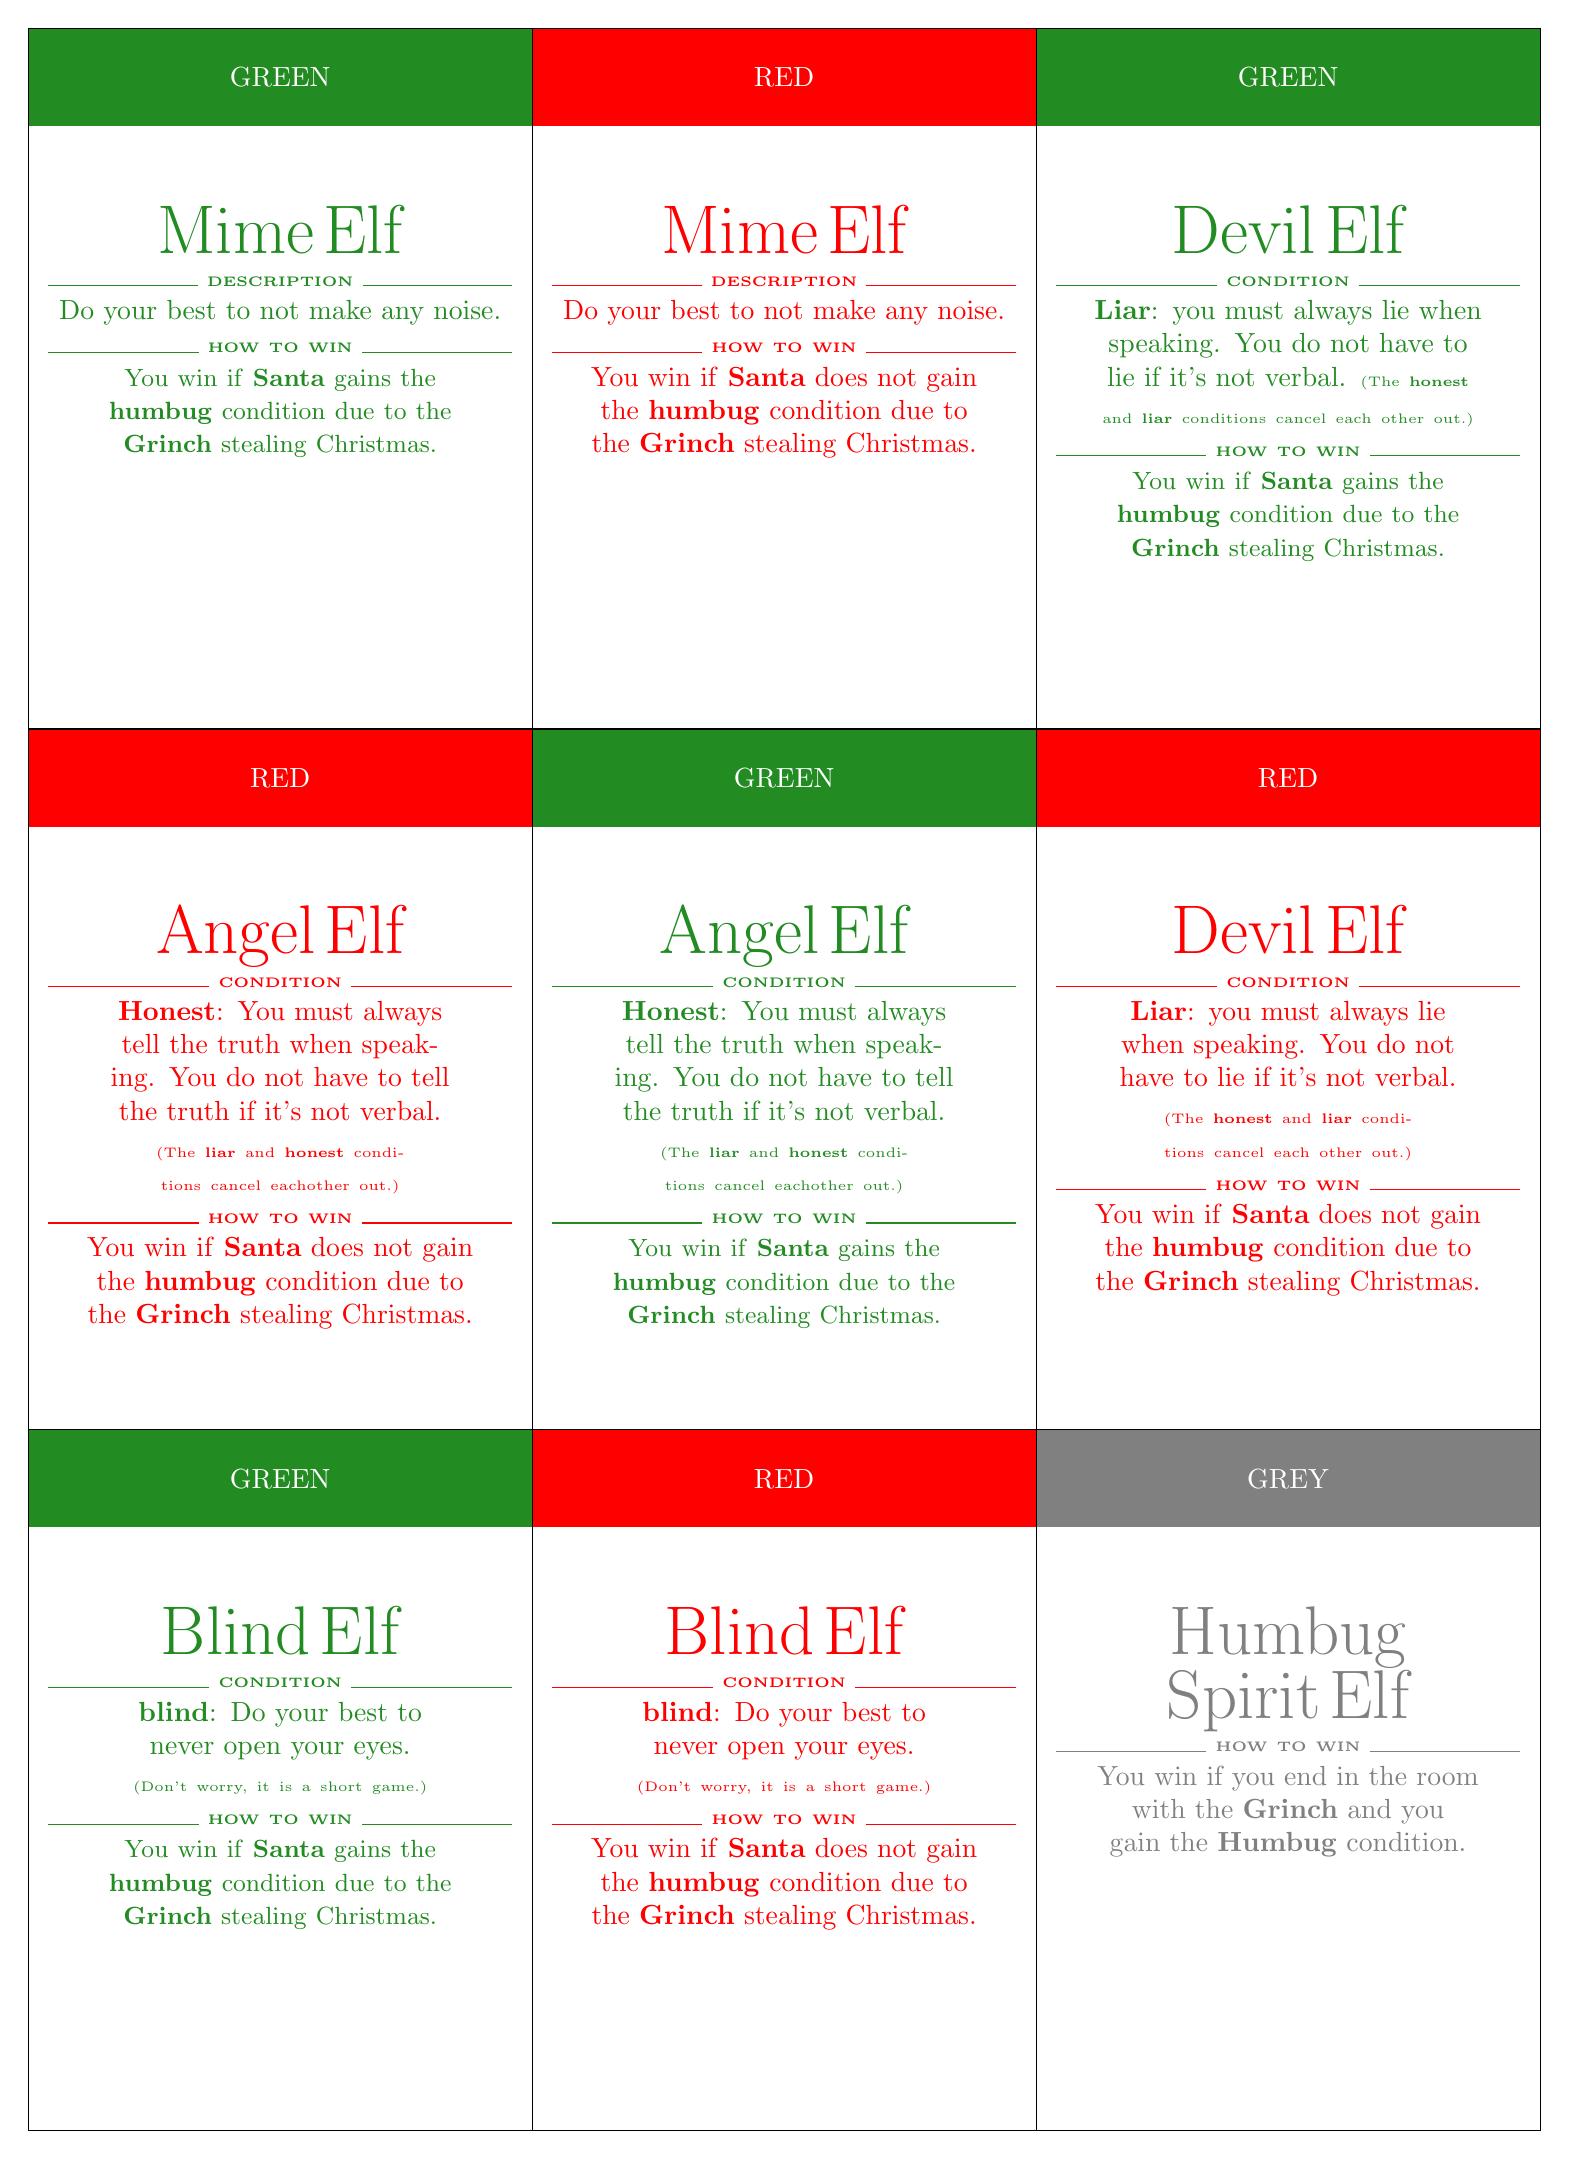
\begin{tikzpicture}[outer sep=0]


% MIME ELF (GREEN TEAM)
\node[teamshare, fill=ForestGreen] (1) at (3.2,26.7) {\HUGE GREEN};
\node[cardtext, text=ForestGreen] at (3.2,24.7) {
	{\Huge Mime Elf}
	\seperatordescription
	Do your best to not make any noise.
	\greenwinsection
};

% MIME ELF (RED TEAM)
\node[teamshare, fill=red] at (9.6,26.7) {\HUGE RED};
\node[cardtext, text=red] at (9.6,24.7) {
	{\Huge Mime Elf}
	\seperatordescription
	Do your best to not make any noise.
	\redwinsection
};

% DEVIL ELF (GREEN TEAM)
\node[teamshare, fill=ForestGreen] at (16,26.7) {\HUGE GREEN};
\node[cardtext, text=ForestGreen] at (16,24.7) {
	{\Huge Devil Elf}
	\seperatorcondition
	\condition{Liar}: you must always lie when speaking. You do not have to lie if it's not verbal.
	\vspace{0.05cm}
	\tiny (The \condition{honest} and \condition{liar} conditions cancel each other out.) \normalsize
	\greenwinsection
};

% ANGEL ELF (RED TEAM)
\node[teamshare, fill=red] at (3.2,17.8) {\HUGE RED};
\node[cardtext, text=red] at (3.2,15.8) {
	{\Huge Angel Elf}
	\seperatorcondition
	\condition{Honest}: You must always tell the truth when speaking. You do not have to tell the truth if it's not verbal.
	\\\vspace{0.05cm}
	\tiny (The \condition{liar} and \condition{honest} conditions cancel eachother out.) \normalsize
	\redwinsection
};

% ANGEL ELF (GREEN TEAM)
\node[teamshare, fill=ForestGreen] at (9.6,17.8) {\HUGE GREEN};
\node[cardtext, text=ForestGreen] at (9.6,15.8) {
	{\Huge Angel Elf}
	\seperatorcondition
	\condition{Honest}: You must always tell the truth when speaking. You do not have to tell the truth if it's not verbal.
	\\\vspace{0.05cm}
	\tiny (The \condition{liar} and \condition{honest} conditions cancel eachother out.) \normalsize
	\greenwinsection
};

% DEVIL ELF (RED TEAM)
\node[teamshare, fill=red] at (16,17.8) {\HUGE RED};
\node[cardtext, text=red] at (16,15.8) {
	{\Huge Devil Elf}
	\seperatorcondition
	\condition{Liar}: you must always lie when speaking. You do not have to lie if it's not verbal.
	\\\vspace{0.05cm}
	\tiny (The \condition{honest} and \condition{liar} conditions cancel each other out.) \normalsize
	\redwinsection
};

% BLIND ELF (GREEN TEAM)
\node[teamshare, fill=ForestGreen] at (3.2,8.9) {\HUGE GREEN};
\node[cardtext, text=ForestGreen] at (3.2,6.9) {
	{\Huge Blind Elf}
	\seperatorcondition
	\condition{blind}: Do your best to never open your eyes.
	\\\vspace{0.05cm}
	\tiny (Don’t worry, it is a short game.) \normalsize
	\greenwinsection
};

% BLIND ELF (RED TEAM)
\node[teamshare, fill=red] at (9.6,8.9) {\HUGE RED};
\node[cardtext, text=red] at (9.6,6.9) {
	{\Huge Blind Elf}
	\seperatorcondition
	\condition{blind}: Do your best to never open your eyes.
	\\\vspace{0.05cm}
	\tiny (Don’t worry, it is a short game.) \normalsize
	\redwinsection
};

% HUMBUG SPIRIT ELF
\node[teamshare, fill=gray] at (16,8.9) {\HUGE GREY};
\node[cardtext, text=gray] at (16,6.9) {
	{\Huge Humbug Spirit Elf}
	\seperatorwin
	You win if you end in the room with the \condition{Grinch} and you gain the \condition{Humbug} condition.
};

\draw (0,0) -- (19.2,0);
\draw (0,8.9) -- (19.2,8.9);
\draw (0,17.8) -- (19.2,17.8);
\draw (0,26.7) -- (19.2,26.7);

\draw (0,0) -- (0,26.7);
\draw (6.4,0) -- (6.4,26.7);
\draw (12.8,0) -- (12.8,26.7);
\draw (19.2,0) -- (19.2,26.7);



\end{tikzpicture}

%Background is not my own. But courtesy of a user on BGG

\includepdf[pages={1}, angle=90]{cardsbackground.pdf}



\noindent 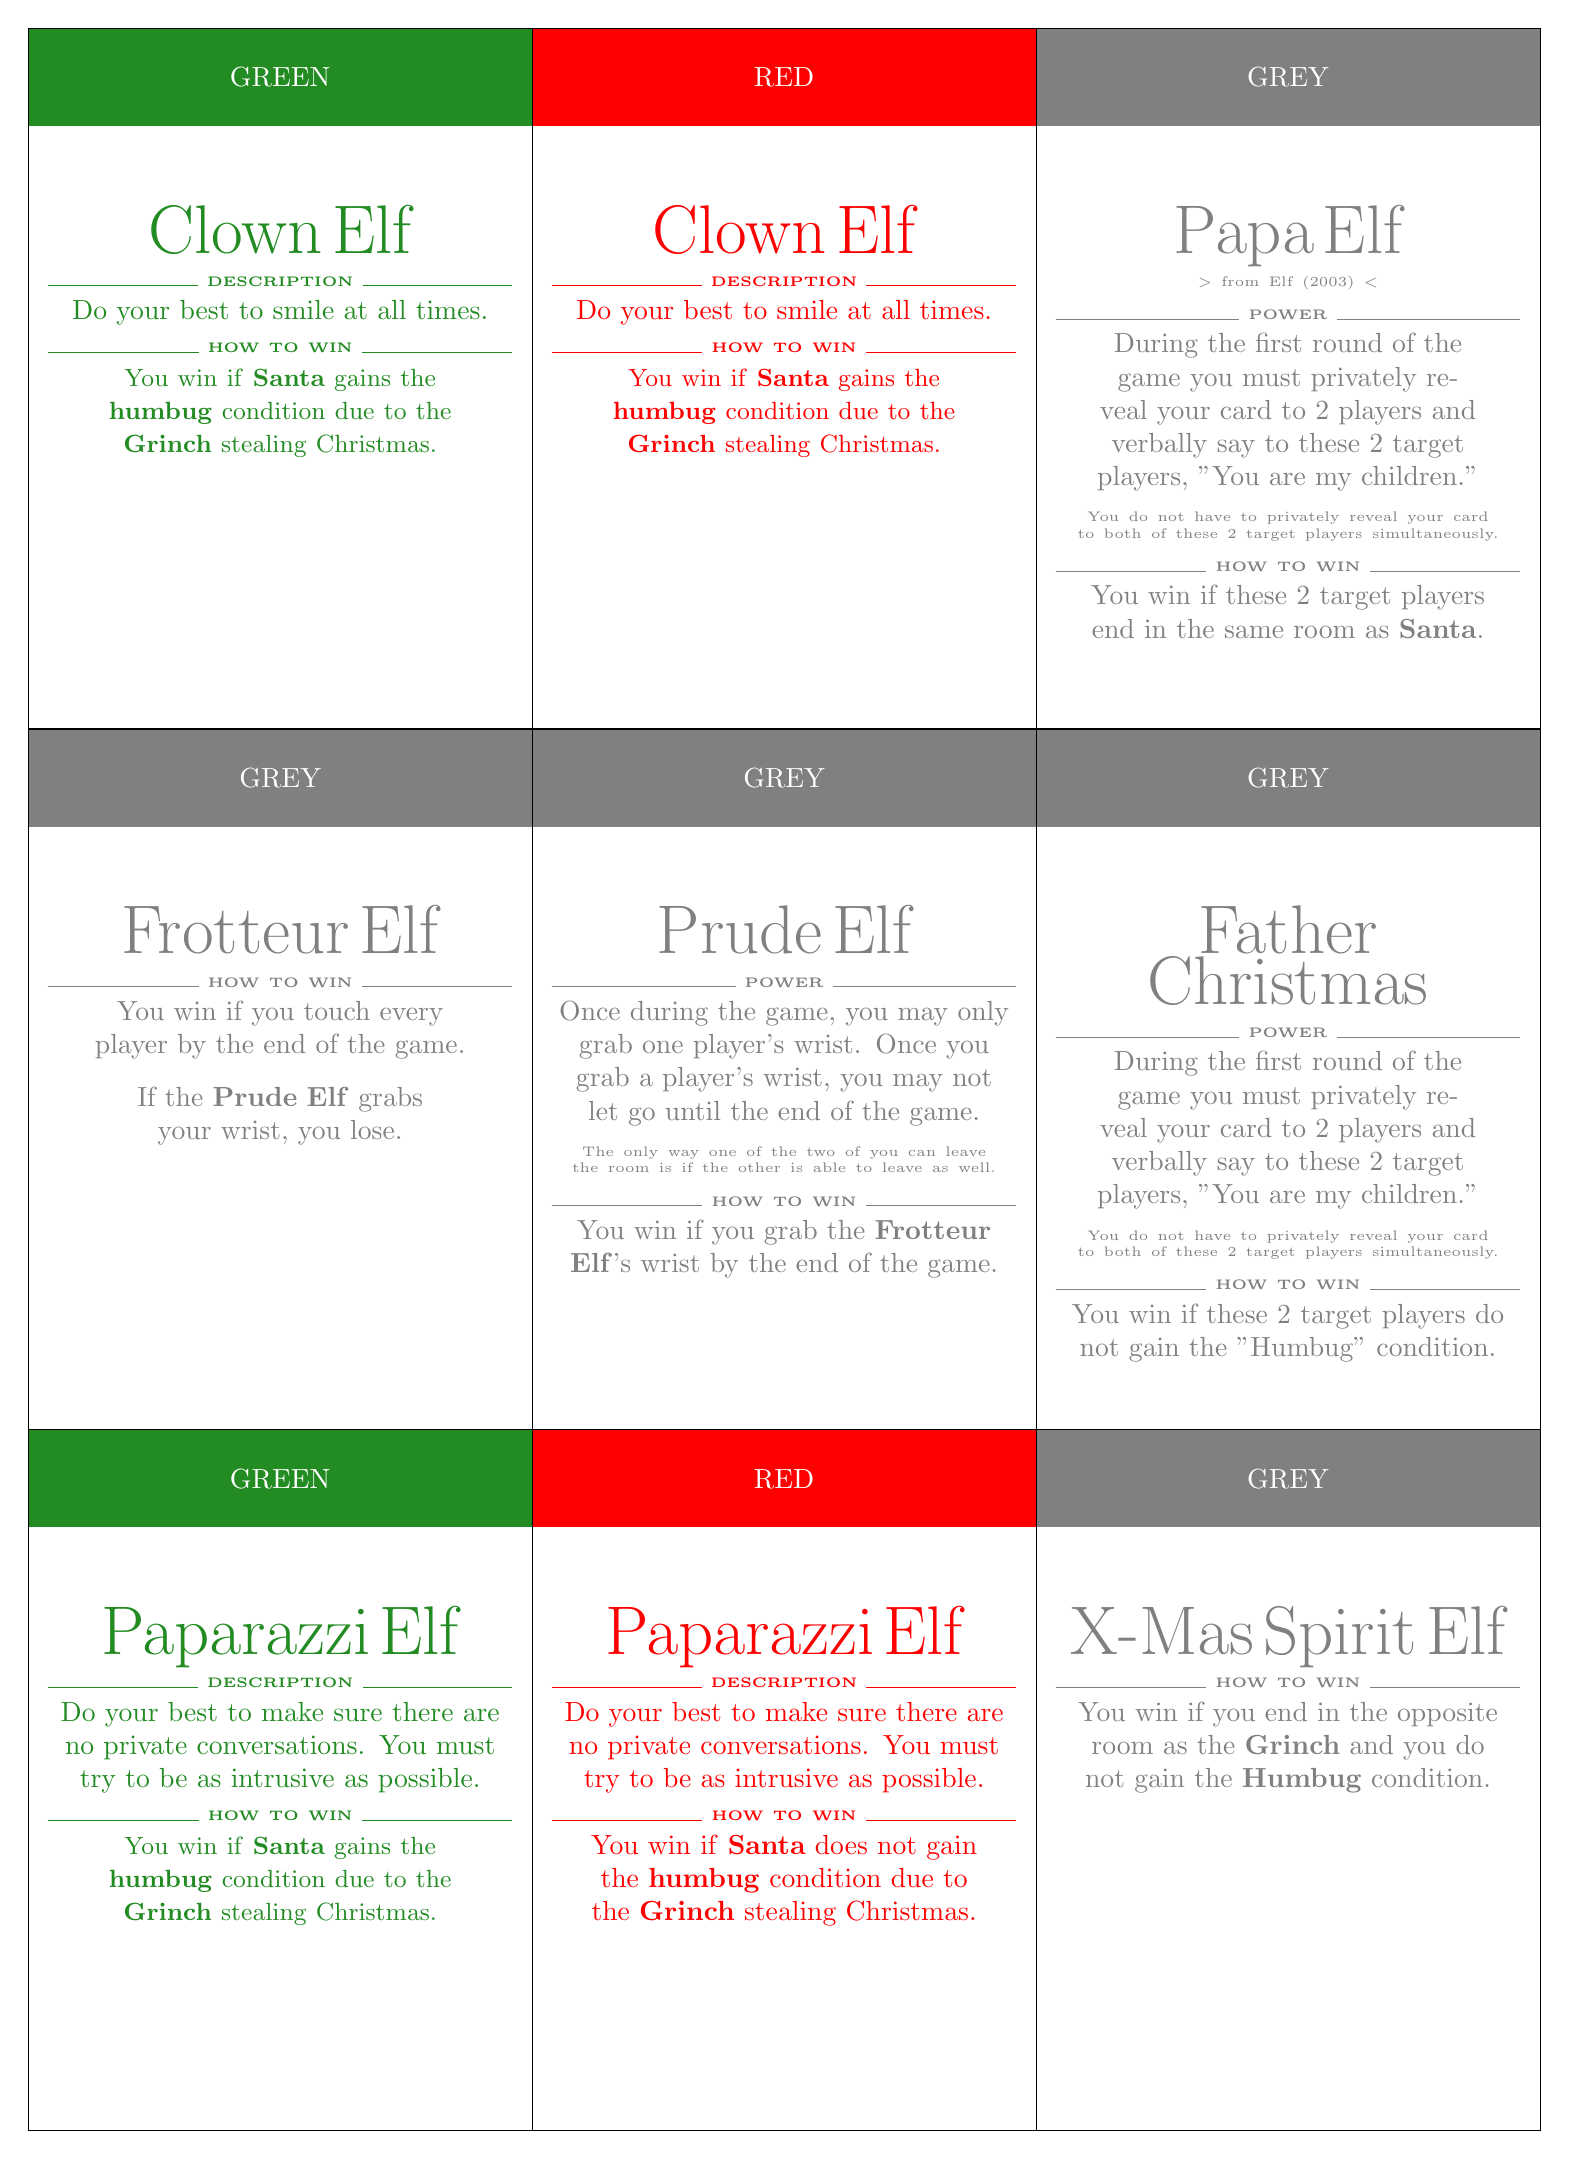
\begin{tikzpicture}[outer sep=0]

% CLOWN ELF (GREEN TEAM)
\node[teamshare, fill=ForestGreen] (1) at (3.2,26.7) {\HUGE GREEN};
\node[cardtext, text=ForestGreen] at (3.2,24.7) {
	{\Huge Clown Elf}
	\seperatordescription
	Do your best to smile at all times.
	\greenwinsection
};

% CLOWN ELF (RED TEAM)
\node[teamshare, fill=red] at (9.6,26.7) {\HUGE RED};
\node[cardtext, text=red] at (9.6,24.7) {
	{\Huge Clown Elf}
	\seperatordescription
	Do your best to smile at all times.
	\greenwinsection
};

% PAPA ELF (aka FATHER)
\node[teamshare, fill=gray] at (16,26.7) {\HUGE GREY};
\node[cardtext, text=gray] at (16,24.7) {
	{\Huge Papa Elf}
	\titlefrom{Elf (2003)}
	\seperatoraction
	During the first round of the game you must privately reveal your card to 2 players and verbally say to these 2 target players, "You are my children.”
	\\\vspace{0.25cm}
	\tiny You do not have to privately reveal your card to both of these 2 target players simultaneously.
	\seperatorwin
	You win if these 2 target players end in the same room as \character{Santa}.
};

% FROTTEUR ELF (RED TEAM)
\node[teamshare, fill=gray] at (3.2,17.8) {\HUGE GREY};
\node[cardtext, text=gray] at (3.2,15.8) {
	{\Huge Frotteur Elf}
	\seperatorwin
	You win if you touch every player by the end of the game.
	\\\vspace{0.25cm}
	If the \condition{Prude Elf} grabs your wrist, you lose.
};

% PRUDE ELF (GREEN TEAM)
\node[teamshare, fill=gray] at (9.6,17.8) {\HUGE GREY};
\node[cardtext, text=gray] at (9.6,15.8) {
	{\Huge Prude Elf}
	\seperatoraction
	Once during the game, you may only grab one player’s wrist. Once you grab a player’s wrist, you may not let go until the end of the game. 
	\\\vspace{0.25cm}
	\tiny The only way one of the two of you can leave the room is if the other is able to leave as well.
	\seperatorwin
	You win if you grab the \condition{Frotteur Elf}'s wrist by the end of the game. 
};

% FATHER CHRISTMAS (aka MOTHER)
\node[teamshare, fill=gray] at (16,17.8) {\HUGE GREY};
\node[cardtext, text=gray] at (16,15.8) {
	{\Huge Father Christmas}
	\seperatoraction
	During the first round of the game you must privately reveal your card to 2 players and verbally say to these 2 target players, "You are my children.”
	\\\vspace{0.25cm}
	\tiny You do not have to privately reveal your card to both of these 2 target players simultaneously.
	\seperatorwin
	You win if these 2 target players do not gain the "Humbug" condition.
};

% PAPARAZZI ELF (GREEN TEAM)
\node[teamshare, fill=ForestGreen] at (3.2,8.9) {\HUGE GREEN};
\node[cardtext, text=ForestGreen] at (3.2,6.9) {
	{\Huge Paparazzi Elf}
	\seperatordescription
	Do your best to make sure there are no private conversations. You must try to be as intrusive as possible.
	\greenwinsection
};

% PAPARAZZI ELF (RED TEAM)
\node[teamshare, fill=red] at (9.6,8.9) {\HUGE RED};
\node[cardtext, text=red] at (9.6,6.9) {
	{\Huge Paparazzi Elf}
	\seperatordescription
	Do your best to make sure there are no private conversations. You must try to be as intrusive as possible.
	\redwinsection
};

% XMAS SPIRIT ELF
\node[teamshare, fill=gray] at (16,8.9) {\HUGE GREY};
\node[cardtext, text=gray] at (16,6.9) {
	{\Huge X-Mas Spirit Elf}
	\seperatorwin
	You win if you end in the opposite room as the \condition{Grinch} and you do not gain the \condition{Humbug} condition.
};

\draw (0,0) -- (19.2,0);
\draw (0,8.9) -- (19.2,8.9);
\draw (0,17.8) -- (19.2,17.8);
\draw (0,26.7) -- (19.2,26.7);

\draw (0,0) -- (0,26.7);
\draw (6.4,0) -- (6.4,26.7);
\draw (12.8,0) -- (12.8,26.7);
\draw (19.2,0) -- (19.2,26.7);



\end{tikzpicture}
%Background is not my own. But courtesy of a user on BGG

\includepdf[pages={1}, angle=90]{cardsbackground.pdf}



\end{document}